\begin{frame}{Modèle des N-Grammes}
\begin{figure}
\centering
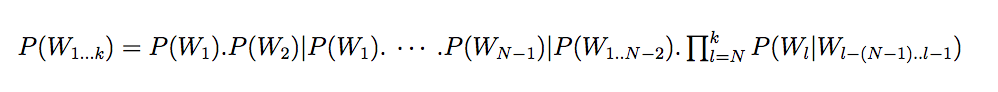
\includegraphics[width=8cm]{images/modele_langage.png}
\end{figure}
\end{frame}

\begin{frame}{Création de Modèle de langage en utilisant CMUCLMTK}
La création d'un Modèle de langage statistique peut se résumer en trois étapes:
\begin{itemize}
\item Collecter des textes
\item Transformer les textes en corpus
\item Transformer le corpus en une distribution de probabilités
\end{itemize}
\end{frame}

